\section{Prospective Benchmark Results}
\label{sec:prospective}

\subsection{Scope and Audit Trail}

The final benchmark contains 11 datasets. Cora, CiteSeer, PubMed, and Coauthor-CS represent citation and co-authorship graphs; Chameleon, Squirrel, Actor, Wisconsin, Cornell, Roman-empire, and Amazon-ratings broaden the structural regimes. Each dataset uses ten fixed seeds, with 60\% of nodes for training, 20\% for validation, and 20\% for testing. The run yields 770 selected-model records and 110 diagnostic records: every unit contains the MLP and six graph architectures, four tuning trials per architecture, explicit split and environment provenance, and one test evaluation after validation selection. The graph and MLP actions therefore search 24 and four trial configurations, respectively; this is a frozen asymmetric-portfolio comparison, not an equal-total-compute comparison. No final-run unit fails.

The execution history contains two documented amendments. First, the v1 feasibility run stops before model training on Texas because one class contains a single node and cannot populate the frozen three-way split. Before comparative assembly or evaluation, an outcome-independent eligibility amendment excludes Texas, assigns a new run identifier, and restarts all remaining datasets from zero without changing models, splits, seeds, thresholds, metrics, or inference. Second, after a blinded wall-clock timeout on Squirrel, an execution-only amendment increases the per-dataset limit from 30 to 90 minutes. No comparative outcome is inspected, and all scientific settings remain unchanged. The completed v2 artifacts retain the amendments and exclude the aborted v1 records from analysis.

Here ``prospective'' refers specifically to newly generated records for the pre-specified primary analysis, produced after the specification and scoring implementation were frozen. Legacy aggregate results inspected during exploratory work are not part of this analysis because they lack consistent paired outcomes and decision-time provenance. The public release provides the frozen snapshot, file digests, and mappings to execution provenance, but it does not expose the private predecessor history; the auditable claim is therefore about the released primary run rather than the entire earlier research timeline.

\subsection{Primary Policy Outcomes}

Graph is the target action in 89 of 110 units, so a selector must be compared with the trivial always-graph policy rather than judged by raw accuracy alone. Table~\ref{tab:prospective_policy_results} reports every frozen policy on identical units. The historical combined diagnostic reaches 55.5\% selection accuracy at 68.2\% coverage. Its covered decisions incur 2.64 percentage points of regret, but the common MLP fallback on 35 abstentions raises full-set regret to 7.46 points.

\begin{table}[t]
\centering
\caption{Prospective Graph-vs-MLP Policy Results on 110 Dataset--Seed Units. Regret is reported in percentage points; selection accuracy uses the common MLP fallback.}
\label{tab:prospective_policy_results}
\small
\begin{tabular}{@{}lccc@{}}
\toprule
Policy & Accuracy (\%) & Coverage (\%) & Regret (pp) \\
\midrule
Combined & 55.5 & 68.2 & 7.46 \\
Always-graph & 80.9 & 100.0 & 0.26 \\
Always-MLP & 19.1 & 100.0 & 9.69 \\
Random 50/50 & 50.0 & 100.0 & 4.97 \\
Homophily-only & 55.5 & 100.0 & 7.46 \\
Degree-only & 37.3 & 100.0 & 6.24 \\
Homophily+degree & 46.4 & 100.0 & 5.80 \\
Two-hop-only & 28.2 & 100.0 & 8.27 \\
Validation selection & 91.8 & 100.0 & 0.22 \\
\bottomrule
\end{tabular}
\end{table}

\begin{figure}[t]
\centering
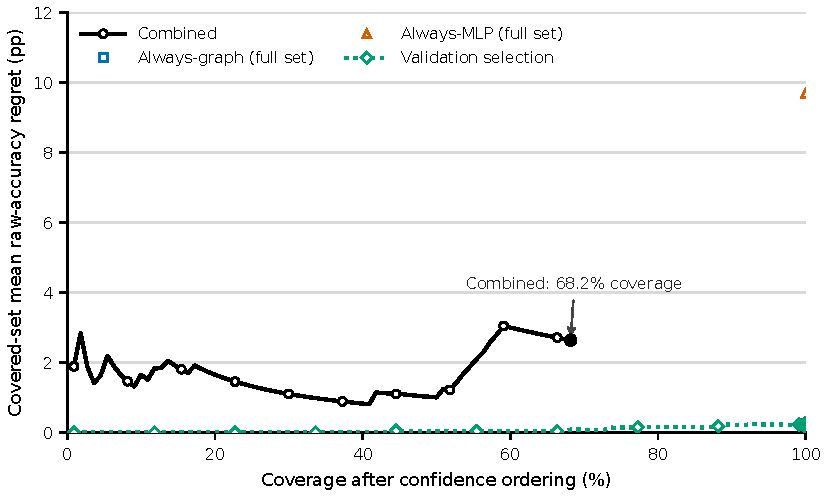
\includegraphics[width=0.82\linewidth]{results/diagnostic/route_a_prospective_v2/analysis/prospective_regret_coverage.pdf}
\caption{Descriptive regret--coverage display from the frozen confidence scores. For Combined and validation selection, coverage increases as lower-confidence eligible decisions enter. Always-graph and always-MLP have constant confidence and therefore appear only as full-set endpoints. The ordinate is covered-set mean raw-accuracy regret, not selection error under the one-point target margin. The Combined curve ends at 68.2\% because 35 units abstain and fallback decisions are not added to this display. The pre-specified primary analysis remains full-set regret with dataset-level inference.}
\label{fig:regret_coverage}
\end{figure}

Always-graph attains 80.9\% selection accuracy and 0.26 points of regret. Direct validation selection attains 91.8\% and 0.22 points, respectively. Homophily-only has the same full-set accuracy and regret as the combined policy after fallback. Although degree-only and homophily-plus-degree reduce descriptive full-set regret relative to Combined, none of the evaluated low-dimensional rules improves on always-graph; under this portfolio and target, they do not demonstrate incremental value in this benchmark.

The equality with homophily-only is not an aggregate coincidence. Combined produces 40 graph, 35 MLP, and 35 abstain actions before fallback. With the frozen MLP fallback, its 110 effective actions exactly match those from the homophily rule. Among the 35 abstentions, 30 have graph as the margin-defined target and 32 have higher raw graph test accuracy; the difference reflects the one-point practical margin. Appendix~\ref{app:action_confusion} reports the complete action-by-target table and distinguishes these targets from positive-regret counts. As a post-hoc descriptive graph-fallback sensitivity, assigning graph rather than MLP to only those abstentions yields 78.2\% selection accuracy and 1.82 points of regret. This remains worse than always-graph and does not replace the frozen MLP-fallback primary result. The \hyperref[app:reproducibility]{record-reconstruction appendix} reports the action counts and regret by dataset, making the concentration of fallback losses explicit.

Table~\ref{tab:fallback_decomposition} decomposes the full-set loss of the rule together with its declared fallback. The 75 covered decisions contribute 1.799 points to the full-set mean, and the 35 MLP-fallback decisions contribute 5.658 points, or 75.876\% of the total regret. The covered-set mean and full-set mean have different denominators; their difference alone is not the fallback contribution.

\begin{table}[t]
\centering
\caption{Descriptive decomposition of Combined with the frozen MLP fallback. Regret entries are percentage points. Each full-set contribution is the sum of regrets in that group divided by all 110 units.}
\label{tab:fallback_decomposition}
\small
\begin{tabular}{@{}lrrr@{}}
\toprule
Decision group & Units & Within-group mean regret & Full-set contribution \\
\midrule
Covered decisions & 75 & 2.638 & 1.799 \\
Abstentions with MLP fallback & 35 & 17.783 & 5.658 \\
\midrule
Total & 110 & 7.457 & 7.457 \\
\bottomrule
\end{tabular}
\end{table}

The observed homophily values also limit what can be learned about the cutoff. The adjacent observed values around $0.50$ are approximately $0.3848$ and $0.7125$. Every threshold strictly between those two unrounded values therefore produces the same 110 actions. The homophily-only versus Combined comparison is an identity after fallback, with difference and interval exactly zero and $p=1$. We retain this comparison in the eight-member Holm family; the current data do not distinguish thresholds within this interval.

Figure~\ref{fig:regret_coverage} shows the precomputed descriptive curves for Combined and validation selection, together with the two constant policies at their identifiable full-set endpoints. Raising confidence within the Combined rule does not reveal a sustained regret region comparable to the low-regret reference policies: its final covered-set regret is 2.64 points at 68.2\% coverage, compared with full-set regrets of 0.26 for always-graph and 0.22 for validation selection. This display is a sensitivity summary only and does not replace the predeclared full-set comparison.

\subsection{Paired Inference and Interpretation}

Relative to the combined diagnostic, the dataset-level mean regret difference is $-7.20$ points for always-graph. Its unadjusted 95\% bootstrap interval is $[-13.17,-1.70]$, with a raw sign-flip $p$-value of $0.015625$. The difference for validation selection is $-7.24$ points, with an unadjusted interval of $[-13.18,-1.78]$ and raw $p=0.03125$. After Holm correction across all eight comparisons, the adjusted values are $0.125$ and $0.21875$. We therefore do not claim multiplicity-adjusted superiority for either reference policy, and we do not treat the non-significant adjusted tests as equivalence.

\paragraph{Structural resolution limitation of the key comparison.}
An exact two-sided sign-flip test with $k\geq1$ nonzero dataset-level differences has a minimum attainable $p$-value of $2^{1-k}$; when $k=0$, $p=1$. For the fixed datasets and diagnostic inputs in this study, Combined and always-graph select graph on Cora, CiteSeer, PubMed, and Coauthor-CS. Their regret differences on these four datasets are therefore identically zero, irrespective of the learned test accuracies. The comparison has at most seven nonzero differences and a raw $p$-value floor of $p_0=0.015625$. Under these fixed diagnostic actions, only the random and validation-selection comparisons can attain raw $p$-values below $p_0$.\footnote{Relative to Combined after the declared fallback, fixed-action disagreements can occur on at most four datasets for always-MLP, zero for homophily-only, six for degree-only, five for homophily+degree, and seven for two-hop-only. These are structural upper bounds on nonzero dataset-level regret differences; with no disagreements, $p=1$.} If always-graph ranks first or second, its Holm multiplier is at least seven; if it ranks third or later, Holm's running maximum is at least $6p_0=0.09375$. Thus rejection at $\alpha=0.05$ is unattainable for this key comparison under the fixed eight-comparison family and realized dataset composition. This is a design limitation, not merely a consequence of the realized test outcomes. In the observed family, the comparison reaches its raw floor at $p=0.015625$ and has the smallest $p$-value, so Holm's first step gives $8\times0.015625=0.125$. The limitation concerns this key comparison and does not imply that every comparison in the family has zero power. Its non-rejection supplies no evidence of equivalence and cannot independently support the operational conclusion below.

The operational conclusion follows the frozen paper-level rule in Section~\ref{sec:protocol}. Combined fails its regret-reduction requirement against always-graph (7.46 versus 0.26 points), independently of the sign-flip resolution limit; the reported unadjusted interval lies in the opposite direction to an incremental-value claim. Selection accuracy alone would hide the magnitude of the loss: the target imbalance makes always-graph strong, while regret shows that the diagnostic's errors are also substantially more costly. Under this protocol the evaluated diagnostics do not demonstrate incremental value in this benchmark. Section~\ref{sec:edge_intervention} provides a separate graph-signal intervention on three citation networks, and Section~\ref{sec:discussion} then discusses a possible diagnostic--portfolio mismatch and its limits.
